In recent decades, foreign direct investment (FDI) global flow has steadily increased, rising to over \$1.5 trillion dollars in 2014. For developing countries, FDI flow is also remarkably robust to global downturn, leading to enthusiastic endorsement by major international organizations as a key factor to economic development (\Cref{fig:globalfdi}).\footnote{http://www.imf.org/external/pubs/ft/fandd/1999/03/mallampa.htm, http://www.weforum.org/reports/foreign-direct-investment-key-driver-trade-growth-and-prosperity-case-multilateral-agreement} This assumption is also shared widely within political science, where much of the literature starts with the assumption that countries want to seek FDI for its many benefits. The question that these works focus on is \textit{how} countries can attract FDI, not \textit{whether} they want to do so \citep{Jensen2003, Li2003, Li2006, Ahlquist2006}.\footnote{Two recent exceptions are \citet{Pinto2013, Pandya2013}, which are the first to investigate the demand for FDI.} 

\begin{figure}[!ht]
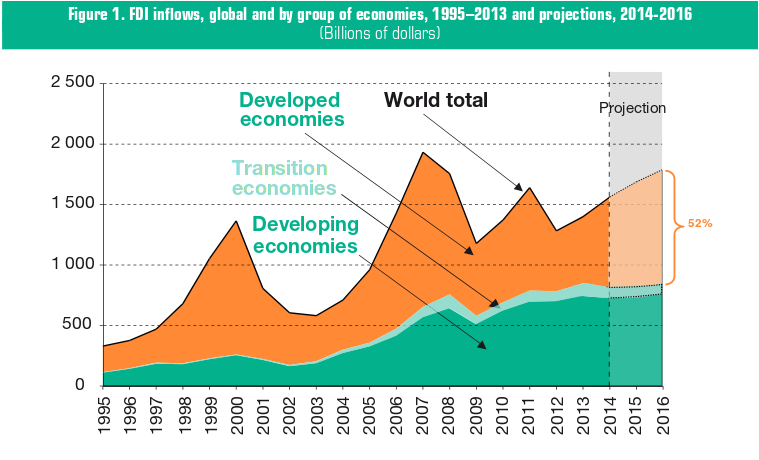
\includegraphics[width=\textwidth, height=\textheight,keepaspectratio]{../figure/global_fdi}
\caption{Source: World Investment Report, 2014}
\label{fig:globalfdi}
\end{figure}

Underlying this mode of thinking is the assumption that FDI brings various benefits to developing countries, including capital and employment. However, the most important promise that FDI holds to growth is the spillover of productivity between foreign firms and domestic firms. This can happen if local firms hire workers that were trained in a foreign firms, improve productivity through backward and forward linkages, or imitate foreign technology. According to growth theory, it is FDI's spillover, not capital or employment, that brings the technological innovation that is requisite for economic growth \citep{Findlay1978}. In this view, FDI is also a public good, providing spillover benefits to the local firms in ways that foreign firms do not take into account in their private calculations. This provides the justification for countries' using investment incentives to rectify the undersupply of FDI, closing the gap between private and social returns. 

Despite this prevailing view, there is little conclusive evidence of FDI having a positive effect on growth \citep{Nair-Reichert2001, Carkovic2002} or poverty reduction \citep{Guerra2009} (\Cref{fig:fdipoverty}). A substantial literature has developed to explain this puzzle, concluding that the growth-enhancing and spillover effect of FDI is conditional on the absorptive capacity of local firms. Cross-nationally, scholars find that FDI is more likely to have a positive growth effect when the technological gap between the local and foreign firms are small \citep{Nunnenkamp2004} and when host countries have strong financial and institutional development \citep{ Durham2004}. Similarly, absorptive capacity, measured by the level of schooling in host economy, conditions the transfer of technology between foreign and local firms across regions in China \citep{Fu2008} and countries in Latin America \citep{Willem2004}.

\begin{figure}[!ht]
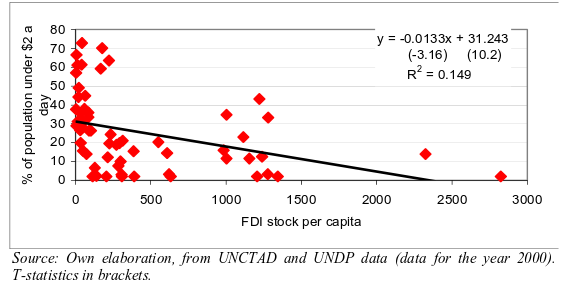
\includegraphics[width=\textwidth, height=\textheight,keepaspectratio]{../figure/fdi_poverty}
\caption{Relationship between FDI and poverty}
\label{fig:fdipoverty}
\end{figure}

Despite the resounding conclusion that the effect of FDI is highly conditional and that investment incentives do not work, why do countries still fixate so much on bringing in FDI instead of developing local absorptive capacity \citep{Blomstrom2002}? For example, Ireland provided foreign investors with lower tax rate, lower land price, and cash grants for R\&D that do not need to be repaid. China also used a tax holiday (two years of no tax and three year of half the normal tax rate) in special economic zones to attract more foreign firms \citep{Telford2001}. We see the same widespread use of investment incentives in Southeast Asia \citep{Fletcher2002}. In Vietnam, the race to offer incentives to foreign firms rages on even among sub-national units, as provincial governments defied the central government's directive and offered extra-legal incentives to FDI firms \citep{Vu2007}. Not only do these measures not work in attracting more FDI, they also deprive countries of revenues that could be spent on improving the local labor quality and investment climate, which are much more conducive to spillover effect and growth.

Thus, my dissertation project focuses on this empirical puzzle: if the positive effect of FDI is uncertain, why is there so much focus on attracting it? If developing absorptive capacity is so crucial to making FDI growth-enhancing, why is it often neglected? To understand this puzzle, I propose that we need to take into account the calculus of government officials, who may be more interested in the potential rents from foreign firms than the spillover and growth-enhancing effect of FDI. This is a potential reason why we often see countries (i.e. government officials) being so enthusiastic about attracting FDI, yet not so passionate about developing the local capacity that enables FDI to actually have a positive effect on growth.

Starting with this empirical puzzle, my project also contributes to various literatures. First, it investigates the collusion of FDI firms and host countries' officials. This is a understudied phenomenon as the existing literature often assumes a foreign firm trying to fend off extortion and harassment from host countries. Second, it examines the political drivers behind private sector development, an issue whose welfare impact is well-known yet whose political determinants are ill-understood. Third, I engage with the decentralization literature in the case study of Vietnam, where I argue that the decision by provincial officials to seek rent from FDI instead of developing the domestic sectors depends on their interest in promotion.
